



\section{Durchführung}
\label{sec:Durchführung}

    \subsection{Aufbau bei einem Druck bis maximal 1 bar}
    Um die Dampfdruchkurve bei $p\leq\qty{1}{\bar}$ zu messen, wird 
    Es befindet sich Wasser in einem Mehrhalskolben, in welchem sich ein ein Thermometer befindet.
    Der Kolben steht auf einer Heizhaube, damit die Temperatur des Wassers regulierbar ist.
    An dem Mehrhalskolben ist außerdem ein Rückflusskühler angeschlossen, der die aufsteigenden Dämpfe daran hindern soll, in das dahinter angeschlossene Manometer zu gelangen.
    Mit diesem kann der Druck des Dampfes gemessen werden.
    Außerdem ist, wie in Abbildung \ref{fig:aufbau1} dargestellt, über eine Woulfsche Flasche eine Wasserstrahlpumpe verbunden.
    Mit dieser lässt sich der Aufbau evakuieren.
    Abgetrennt ist dieser durch einen Absperrhahn zur Woulfschen Flasche, welche wiederum über ein Drosselventil vom Rest des Aufbaus abgetrennt ist.
    Der Zweck der Woulfschen Flasche ist, den hinter dem Drosselventil liegenden Teil des Aufbaus vor möglichem Eindringen von kaltem Wasser zu schützen.
    Zudem ist ein Belüftungsventil am der Apparetur angeschlossen.

    \begin{figure}[H]
        \centering
        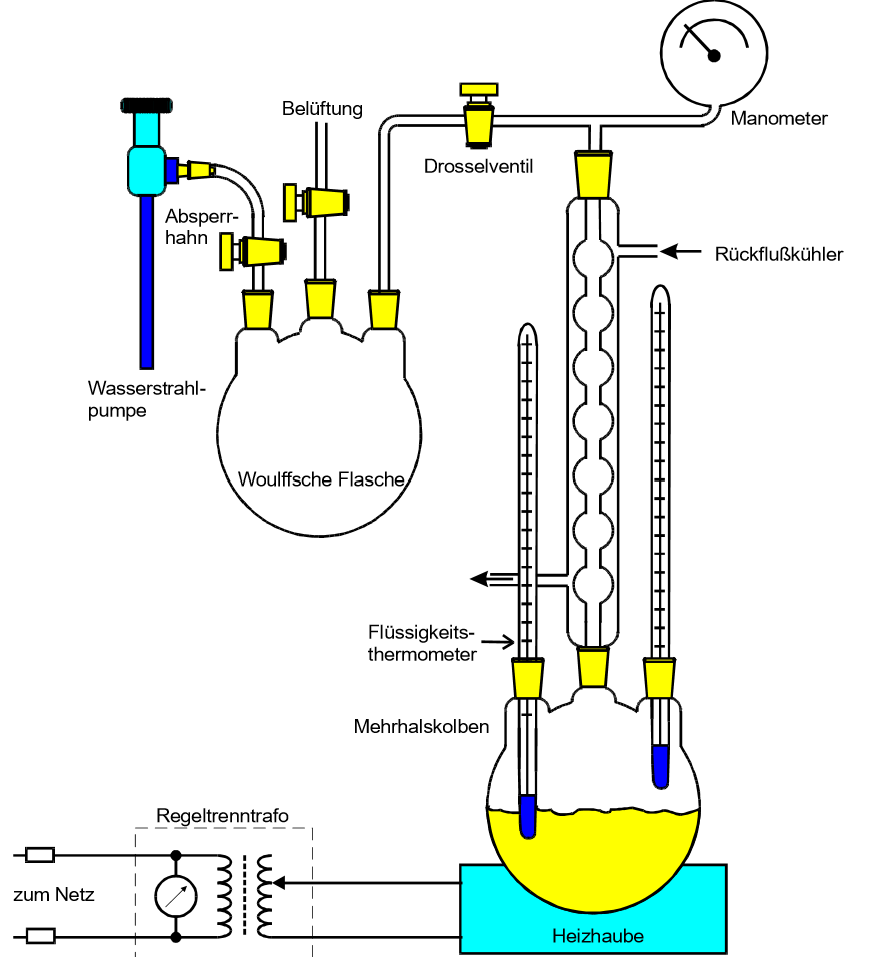
\includegraphics[height=9cm]{Bilder/Aufbau1.png}
        \label{fig:aufbau1}
        \caption{Abgebildet ist ein Modell des Aufbaus zur Messung der Verdampfungswärme bei einem Druck bis maximal 1 bar.}
    \end{figure}

    \subsection{Durchführung bei einem Druck bis maximal 1 bar}
    Zu Beginn wird der Atmosphärendruch mit dem Manometer gemessen.
    Der Aufbau wird danach mithilfe der Wasserstrahlpumpe evakuiert.
    Dabei ist der Absperrhahn und das Drosselventil geöffnet. 
    Das Lüftungsventil bleibt geschlossen, während das Experiment durchgeführt wird. 
    Dabei wird gewartet, bis der kleinstmögliche Druck erreicht wird.
    Danach wird der Absperrhahn und das Drosselventil geschlossen.
    Zur selben Zeit werden dann die Wasserzufuhr des Rückflusskühlers und die Heizhaube eingeschaltet.
    Nun werden Wertepaare für den Dampfdruck und die Temperatur abgelesen, bis der Druck 1 bar erreicht.

    \subsubsection{Aufbau bei einem Druck größer als 1 bar}
    Dargestellt ist der Aufbau in Abbildung \ref{fig:aufbau2}
    In einem Stahlbolzen befindet sich Wasser.
    An dem Bolzen sind Heizwicklungen angebracht, um diesen zu erhitzen.
    Um die Siedetemperatur zu messen befindet sich ein Thermometer im Wasser.
    Über ein U-Rohr ist dann ein Drucksensor verbunden, um auch hier den Druck des Systems zu messen.%%Kühlflüssigkeit?

    \begin{figure}[H]
        \centering
        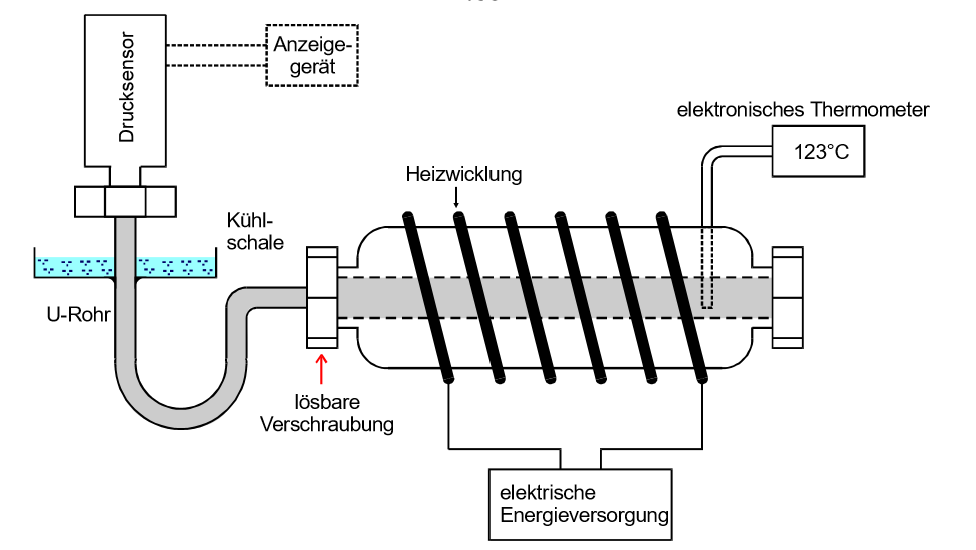
\includegraphics[height=7cm]{Bilder/Aufbau2.png}
        \label{fig:aufbau2}
        \caption{Dies ist der schematische Aufbau zur Messung der Verdampfungswärme bei einem Druck größer als 1 bar.}
    \end{figure}

    \subsection{Durchführung bei einem Druck größer als 1 bar}
    Mit den Heizwicklungen wird der Stahlbolzen langsam augeheitzt.
    Dabei werden auch hier Wertepaare für Druck und Temperatur abgelesen.